\documentclass[aspectratio=169,10pt,t]{beamer}
\usetheme{faeder}

\usepackage{pgfplots}
\pgfplotsset{compat=1.18}
\usepackage{hyperref}
\hypersetup{colorlinks=true,urlcolor=fsTeal,linkcolor=fsNavy}

\graphicspath{{figures/}}
\newcommand{\modeldir}{../../models}
\newcommand{\yes}{{\color{fsGreen}\checkmark}}
\newcommand{\no}{{\color{fsAccent}$\times$}}

% Shared plot style
\pgfplotsset{
  fsplot/.style={
    width=\linewidth, height=0.62\linewidth,
    axis lines=left, tick label style={font=\scriptsize},
    label style={font=\footnotesize}, legend style={font=\scriptsize,draw=none,fill=none},
    legend cell align=left, every axis plot/.append style={line width=1.2pt},
    xlabel={time (min)}, ymin=0, enlarge x limits=false,
  },
  cycle list={{fsNavy},{fsAccent},{fsTeal},{fsGold},{fsGreen},{fsGray}},
}

% Molecule diagrams
\tikzset{
  molbox/.style={draw=black!55,rounded corners=3pt,line width=0.6pt,
                 minimum height=7mm,font=\small\bfseries,inner xsep=3mm},
  site/.style={circle,draw=black!55,fill=white,inner sep=0pt,minimum size=4mm,
               font=\tiny\bfseries,line width=0.5pt},
  psite/.style={site,fill=fsAccent,text=white},
  bond/.style={line width=1.3pt,black!70},
  callout/.style={font=\scriptsize,text=fsGray,align=left},
  pointer/.style={-{Stealth[length=1.6mm]},fsGray,line width=0.5pt},
}

\title{Rule-Based Modeling of Cell Signaling}
\subtitle{Module 2: Molecular structure and combinatorial complexity}
\author{Jim Faeder}
\institute{MSCBIO 2025 \textperiodcentered{} Introduction to Bioinformatics Programming in Python}
\date{Fall 2026}

\begin{document}

% ======================================================================
\begin{frame}[plain]
  \titlepage
\end{frame}

\begin{frame}{Goals for this module}
  By the end of this module you should be able to
  \begin{enumerate}
    \setlength\itemsep{1.5mm}
    \item explain why multi-site proteins lead to \hl{combinatorial complexity}
    \item represent molecules with \hl{components}, \hl{states}, and \hl{bonds} in BNGL
    \item read and write \hl{patterns}, and use them to define observables
    \item write \hl{reaction rules} and predict which reactions a rule generates
    \item describe how BioNetGen \hl{generates a network} from rules, and when
          network-free simulation is needed instead
  \end{enumerate}
\end{frame}

% ======================================================================
\section{From species to molecules}

\begin{frame}[fragile]{Where Module 1 left off}
  \begin{columns}[T]
    \begin{column}{0.5\textwidth}
      Our cytokine--STAT--SOCS model had \textbf{12 species}, each named by hand:
      \vskip1mm
      \centering
      \small
      \begin{tabular}{llll}
        L & R & LR & S \\
        LRS & LRS$_\mathsf{p}$ & S$_\mathsf{p}$ & G \\
        GS$_\mathsf{p}$ & mSOCS & SOCS & LR$\cdot$SOCS
      \end{tabular}
      \vskip3mm
      \raggedright
      To get total pSTAT we had to list every species that contains it:
\begin{lstlisting}[language=bngl]
Molecules pSTAT LRSp Sp GSp
\end{lstlisting}
    \end{column}
    \begin{column}{0.46\textwidth}
      \begin{block}{Assumptions we made}
        \small
        \begin{itemize}
          \item Ligand only leaves an empty receptor
          \item SOCS and STAT compete for one receptor site
          \item The receptor is a single chain
          \item STAT acts as a monomer with one phosphosite
        \end{itemize}
      \end{block}
      \vskip1mm
      {\small Each of these is false for real cytokine receptors. Relaxing any of them
      requires new species, and new copies of every reaction they take part in.}
    \end{column}
  \end{columns}
\end{frame}

\begin{frame}{Signaling proteins have many interaction sites}
  \begin{columns}[c]
    \begin{column}{0.52\textwidth}
      \centering
      \resizebox{\linewidth}{!}{%
      \begin{tikzpicture}[x=1cm,y=1cm]
        % STAT domain cartoon
        \foreach \xa/\wa/\col/\lab in {0/1.1/fsNavy!25/N-term, 1.1/1.4/fsTeal!25/coiled-coil,
                                 2.5/1.2/fsGold!35/DNA binding, 3.7/0.8/fsGray!20/linker,
                                 4.5/0.9/fsGreen!30/SH2, 5.4/0.9/fsAccent!20/TAD}
          {\draw[black!55,fill=\col] (\xa,0) rectangle ++(\wa,0.6);
           \pgfmathsetmacro{\xm}{\xa+\wa/2}
           \node[font=\tiny,align=center] at (\xm,0.3) {\lab};}
        \node[psite] (y) at (5.55,0.95) {P};
        \node[font=\tiny,above=0pt of y] {Y705};
        \node[psite] (s) at (6.05,0.95) {P};
        \node[font=\tiny,above=0pt of s] {S727};
        \node[font=\small\bfseries,anchor=east] at (-0.1,0.3) {STAT3};
        \draw[decorate,decoration={brace,mirror,amplitude=3pt},black!50] (0,-0.1) -- (2.5,-0.1)
          node[midway,below=2pt,font=\tiny,text=fsGray] {dimerization, nuclear transport};
        \draw[decorate,decoration={brace,mirror,amplitude=3pt},black!50] (4.5,-0.1) -- (5.4,-0.1)
          node[midway,below=2pt,font=\tiny,text=fsGray,align=center] {binds receptor\\pTyr};
      \end{tikzpicture}}
      \vskip4mm
      \begin{tikzpicture}[x=1cm,y=1cm]
        \node[font=\small] at (0,0) {$n$ independent two-state sites};
        \node[font=\small] at (0,-0.55) {$\Rightarrow\; 2^n$ possible states of one molecule};
        \node[font=\small,text=fsGray] at (0,-1.1) {and complexes multiply the counts of their parts};
      \end{tikzpicture}
    \end{column}
    \begin{column}{0.44\textwidth}
      \small
      \begin{itemize}
        \setlength\itemsep{1.5mm}
        \item Each protein has several \textbf{binding domains} and
              \textbf{modification sites}.
        \item Sites can be occupied or modified \emph{in combination}.
        \item Most interactions depend on only one or two sites: SOCS binding does
              not care whether S727 is phosphorylated.
        \item Naming every combination is \hl{combinatorial complexity}: a few
              interactions imply a huge number of species.
      \end{itemize}
    \end{column}
  \end{columns}
\end{frame}

\begin{frame}{Combinatorial complexity in a realistic model of EGFR signaling}
  \begin{columns}[c]
    \begin{column}{0.55\textwidth}
      A model of the ErbB receptor family with its known binding partners:
      \vskip2mm
      \begin{itemize}
        \item ErbB3:ErbB1 dimer: $> 3.8\times10^{9}$ states
        \item ErbB1:ErbB1 dimer: $> 5.5\times10^{10}$ states
      \end{itemize}
      \vskip3mm
      Yet the model is built from a manageable number of \hl{rules}, in the tens to
      hundreds.
    \end{column}
    \begin{column}{0.42\textwidth}
      \centering
      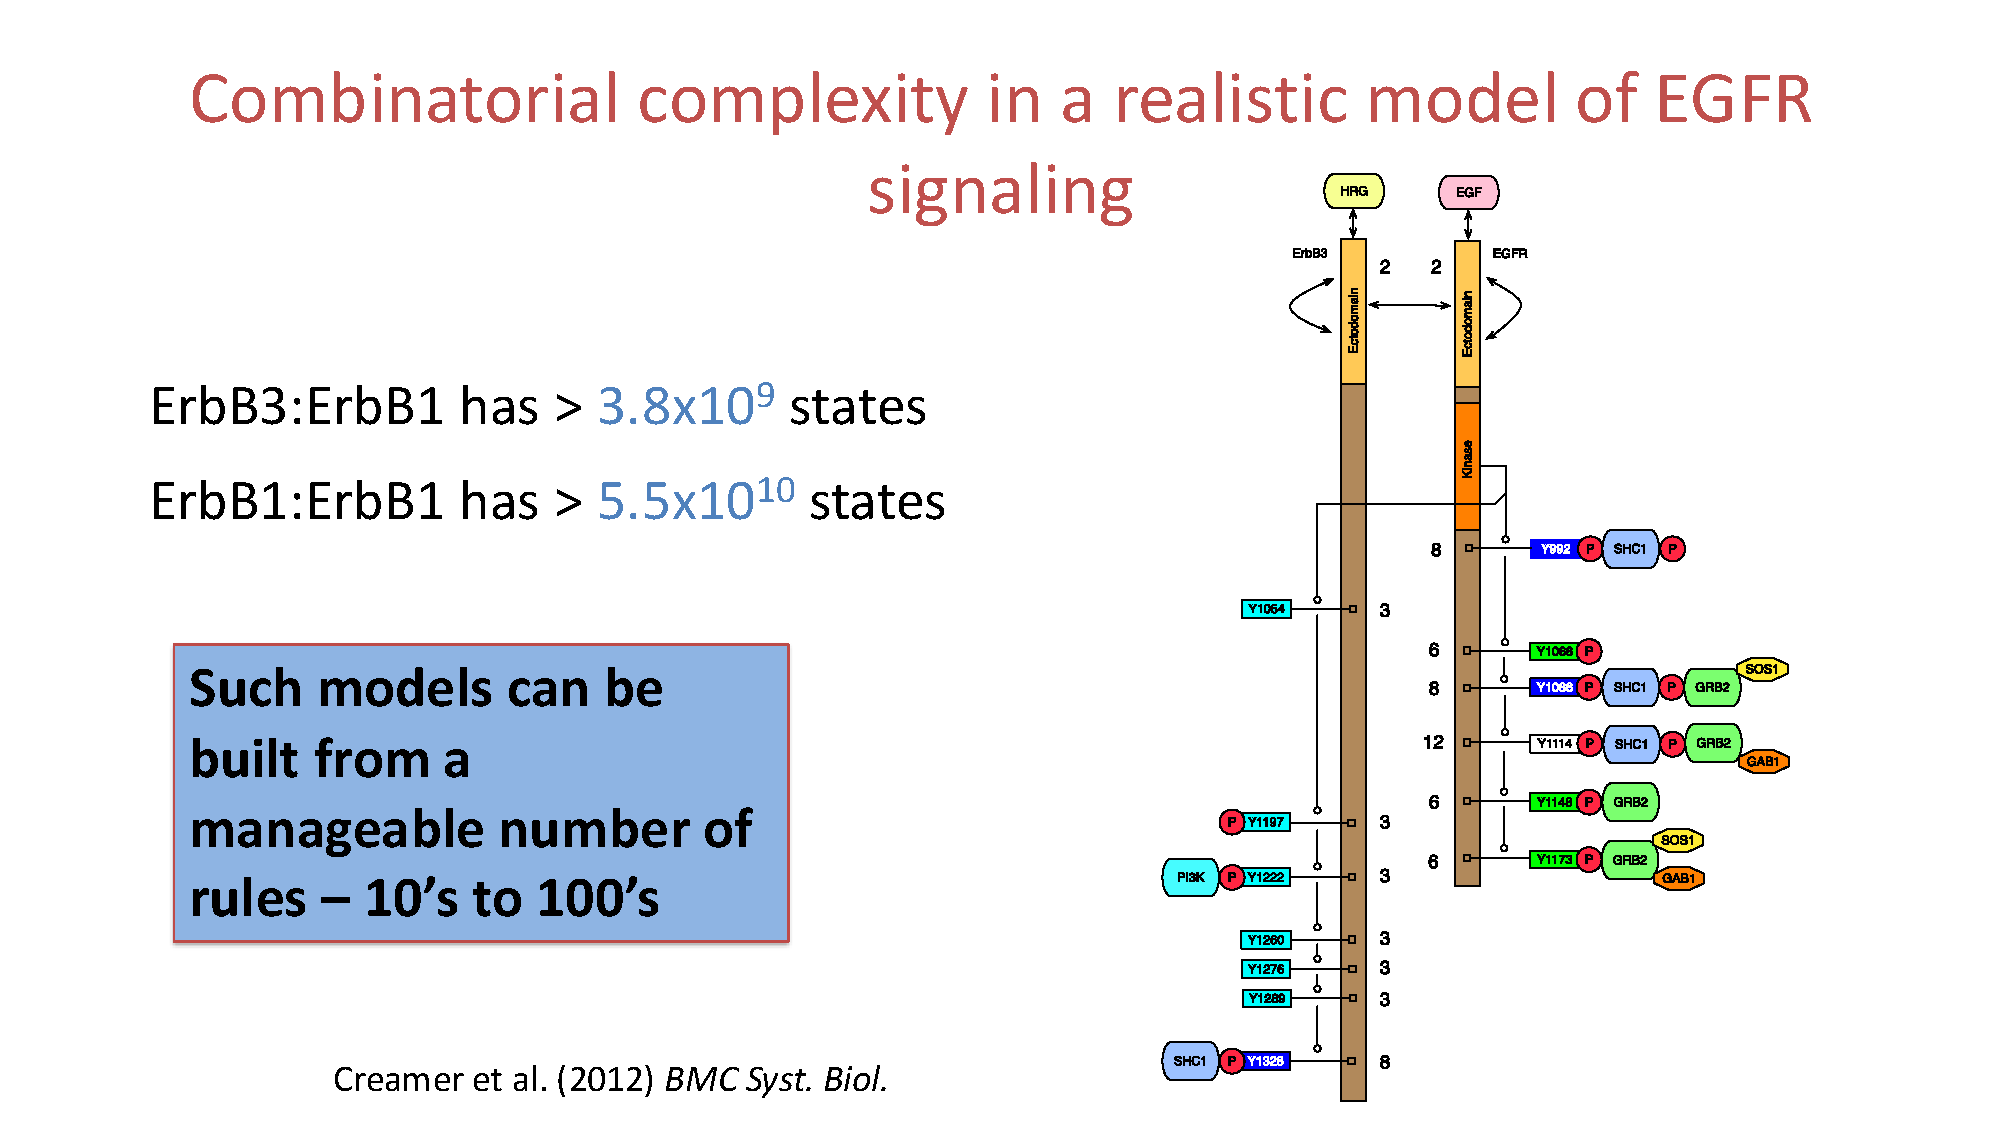
\includegraphics[height=0.72\textheight,trim=548 50 95 80,clip]{creamer_2012_egfr.pdf}
    \end{column}
  \end{columns}
  \source{Creamer et al., \emph{BMC Syst.\ Biol.}\ \textbf{6}, 107 (2012)}
\end{frame}

% ======================================================================
\section{Structured molecules in BNGL}

\begin{frame}[fragile]{Molecules have components, and components can have states}
  \begin{columns}[c]
    \begin{column}{0.5\textwidth}
      \centering
      \begin{tikzpicture}[x=1cm,y=1cm]
        \node[molbox,fill=fsGreen!25,minimum width=2.6cm] (S) at (0,0) {S};
        \node[site] (r) at ($(S.north)$) {r};
        \node[site] (Y) at ($(S.east)$) {Y};
        \node[site] (g) at ($(S.south)$) {g};
        \node[callout,anchor=west] (cr) at (1.9,0.95) {component \code{r}:\\binds receptor};
        \draw[pointer] (cr.west) -- (r.east);
        \node[callout,anchor=west] (cY) at (2.0,0) {component \code{Y}:\\state \code{0} or \code{P}};
        \draw[pointer] (cY.west) -- (Y.east);
        \node[callout,anchor=west] (cg) at (1.9,-0.95) {component \code{g}:\\binds DNA};
        \draw[pointer] (cg.west) -- (g.east);
        \node[callout,anchor=east] (cm) at (-1.7,0.6) {molecule\\name};
        \draw[pointer] (cm.east) -- (S.west);
      \end{tikzpicture}
      \vskip4mm
\begin{lstlisting}[language=bngl]
begin molecule types
  S(r,Y~0~P,g)
end molecule types
\end{lstlisting}
    \end{column}
    \begin{column}{0.46\textwidth}
      \small
      \begin{itemize}
        \setlength\itemsep{1.5mm}
        \item A \textbf{molecule} is a named object with a list of \textbf{components}
              in parentheses.
        \item Components represent \textbf{binding sites} or
              \textbf{modification sites}.
        \item \code{\textasciitilde} lists the allowed \textbf{states} of a component:
              \code{Y\textasciitilde0\textasciitilde P}.
        \item A component can have both a state and a bond.
        \item A molecule with no components, \code{mSOCS()}, is just a species name,
              as in Module 1.
      \end{itemize}
    \end{column}
  \end{columns}
\end{frame}

\begin{frame}[fragile]{Complexes are molecules joined by bonds}
  \begin{columns}[c]
    \begin{column}{0.42\textwidth}
      \centering
      \begin{tikzpicture}[x=1cm,y=1cm]
        \node[molbox,fill=fsGold!40,minimum width=1.4cm] (L) at (0,2.2) {L};
        \node[site] (Lr) at (L.south) {r};
        \node[molbox,fill=fsNavy!20,minimum width=1.8cm] (R) at (0,0.9) {R};
        \node[site] (Rl) at (R.north) {l};
        \node[site] (Rs) at (R.south) {s};
        \node[molbox,fill=fsGreen!25,minimum width=2.2cm] (S) at (0,-0.4) {S};
        \node[site] (Sr) at (S.north) {r};
        \node[psite] (SY) at (S.east) {P};
        \node[site] (Sg) at (S.south) {g};
        \draw[bond] (Lr) -- (Rl) node[midway,right=3pt,font=\tiny\bfseries,text=fsAccent] {1};
        \draw[bond] (Rs) -- (Sr) node[midway,right=3pt,font=\tiny\bfseries,text=fsAccent] {2};
      \end{tikzpicture}
    \end{column}
    \begin{column}{0.55\textwidth}
      The Module 1 species LRS$_\mathsf{p}$ written with structure:
\begin{lstlisting}[language=bngl]
L(r!1).R(l!1,s!2).S(r!2,Y~P,g)
\end{lstlisting}
      \small
      \begin{itemize}
        \setlength\itemsep{1.2mm}
        \item \code{.} joins molecules in the same complex.
        \item \code{!1} marks one end of a bond; the matching \code{!1} is the other end.
              Bond labels only need to be unique within a species.
        \item A component with no \code{!} is \textbf{free}: \code{g} above.
        \item A species is now a \hl{graph}: molecules are nodes, bonds are edges.
              BioNetGen recognizes when two strings describe the same graph.
      \end{itemize}
    \end{column}
  \end{columns}
\end{frame}

\begin{frame}[fragile]{Patterns select sets of species}
  A \textbf{pattern} lists only the parts of a complex you care about.
  \hl{Don't write, don't care}: anything not mentioned can be in any state.
  \vskip2mm
  \centering
  \small
  \begin{tabular}{@{}lccccccl@{}}
    \toprule
    pattern & LR & LRS & LRS$_\mathsf{p}$ & S$_\mathsf{p}$ & GS$_\mathsf{p}$ & LR$\cdot$SOCS & meaning \\
    \midrule
    \code{S(Y\textasciitilde P)}   & \no  & \no  & \yes & \yes & \yes & \no  & any phosphorylated STAT \\
    \code{S(r,Y\textasciitilde P)} & \no  & \no  & \no  & \yes & \yes & \no  & phosphorylated, not on a receptor \\
    \code{S(r!+)}                  & \no  & \yes & \yes & \no  & \no  & \no  & STAT bound via \code{r} \\
    \code{R(l!+)}                  & \yes & \yes & \yes & \no  & \no  & \yes & ligand-bound receptor \\
    \code{R(l!+,s)}                & \yes & \no  & \no  & \no  & \no  & \no  & \ldots{} with docking site free \\
    \code{R(s!+)}                  & \no  & \yes & \yes & \no  & \no  & \yes & docking site occupied \\
    \bottomrule
  \end{tabular}
  \vskip3mm
  \raggedright
  \begin{itemize}
    \item \code{!+} \enspace bound to anything \qquad
          \code{!?} \enspace bound or not \qquad
          no \code{!} \enspace must be free
    \item Matching is done on the graph, so the pattern can match a molecule anywhere
          inside a complex.
  \end{itemize}
\end{frame}

\begin{frame}[fragile]{Observables are patterns}
  \begin{columns}[T]
    \begin{column}{0.48\textwidth}
      \textbf{Module 1}: list every species by hand
\begin{lstlisting}[language=bngl]
Molecules pSTAT LRSp Sp GSp
\end{lstlisting}
      \vskip2mm
      \textbf{Module 2}: describe the property
\begin{lstlisting}[language=bngl]
Molecules pSTAT S(Y~P)
\end{lstlisting}
      \small
      The pattern keeps working when we add new complexes containing pSTAT.
      No observable needs to be rewritten.
    \end{column}
    \begin{column}{0.48\textwidth}
      \begin{block}{\code{Molecules} vs.\ \code{Species}}
        \small
        \begin{itemize}
          \item \code{Molecules} counts every \emph{match}. A STAT dimer with two
                pTyr contributes 2 to \code{S(Y\textasciitilde P)}.
          \item \code{Species} counts each matching \emph{complex} once.
        \end{itemize}
\begin{lstlisting}[language=bngl]
Species pSTATdimer S(d!1).S(d!1)
\end{lstlisting}
      \end{block}
    \end{column}
  \end{columns}
\end{frame}

\begin{frame}[fragile]{Rules transform patterns}
\begin{lstlisting}[language=bngl,basicstyle=\ttfamily\small]
Sbind:  R(l!+,s) + S(r,Y~0) <-> R(l!+,s!1).S(r!1,Y~0)  kSon, kSoff
\end{lstlisting}
  \vskip1mm
  \begin{columns}[T]
    \begin{column}{0.5\textwidth}
      \small
      \begin{itemize}
        \setlength\itemsep{1.2mm}
        \item \textbf{Reactant patterns} (left) say what must be present:
              a ligand-bound receptor with a free docking site, and an
              unphosphorylated STAT with a free \code{r} site.
        \item \textbf{Product patterns} (right) say what changes:
              a bond forms between \code{s} and \code{r}.
        \item Everything not mentioned is carried along unchanged.
        \item Rates follow mass action, with the \emph{rule's} rate constant.
      \end{itemize}
    \end{column}
    \begin{column}{0.46\textwidth}
      \begin{block}{What a rule can do}
        \small
        \begin{tabular}{@{}ll@{}}
          form a bond     & \code{A(b) + B(a) -> A(b!1).B(a!1)} \\
          break a bond    & \code{A(b!1).B(a!1) -> A(b) + B(a)} \\
          change a state  & \code{S(Y\textasciitilde0) -> S(Y\textasciitilde P)} \\
          make a molecule & \code{G(s!+) -> G(s!+) + mSOCS()} \\
          delete one      & \code{SOCS(r) -> 0}
        \end{tabular}
      \end{block}
    \end{column}
  \end{columns}
\end{frame}

% ======================================================================
\section{The Module 1 model as rules}

\begin{frame}[fragile]{Molecule types, seed species, and observables}
  \begin{columns}[T]
    \begin{column}{0.56\textwidth}
\begin{lstlisting}[language=bngl,basicstyle=\ttfamily\footnotesize]
begin molecule types
  L(r)
  R(l,s)
  S(r,Y~0~P,g)
  G(s)
  mSOCS()
  SOCS(r)
end molecule types
begin seed species
  L(r)        L0
  R(l,s)      R0
  S(r,Y~0,g)  S0
  G(s)        G0
end seed species
begin observables
  Molecules pSTAT  S(Y~P)
  Molecules SOCS   SOCS()
end observables
\end{lstlisting}
    \end{column}
    \begin{column}{0.4\textwidth}
      \small
      \begin{itemize}
        \setlength\itemsep{1.5mm}
        \item Six molecule types replace twelve species names.
        \item \textbf{Seed species} are the complexes present at $t=0$. Every other species
              is generated from them by the rules.
        \item The receptor has one docking site \code{s} that STAT and SOCS compete for.
              This is the Module 1 assumption.
      \end{itemize}
      \vskip1mm
      {\scriptsize File: \code{models/stat\_rbm1\_rules.bngl}}
    \end{column}
  \end{columns}
\end{frame}

\begin{frame}[fragile]{The rules}
\begin{lstlisting}[language=bngl,basicstyle=\ttfamily\footnotesize]
LRbind:     L(r) + R(l,s) <-> L(r!1).R(l!1,s)              kon, koff
Sbind:      R(l!+,s) + S(r,Y~0) <-> R(l!+,s!1).S(r!1,Y~0)  kSon, kSoff
Sact:       R(s!1).S(r!1,Y~0) -> R(s!1).S(r!1,Y~P)         kact
Srelease:   R(s!1).S(r!1,Y~P) -> R(s) + S(r,Y~P)           kdiss
Sdephos:    S(r,g,Y~P) -> S(r,g,Y~0)                       kdephos
Gbind:      S(r,Y~P,g) + G(s) <-> S(r,Y~P,g!1).G(s!1)      kGon, kGoff
Transcribe: G(s!+) -> G(s!+) + mSOCS()                     ktx
mRNAdeg:    mSOCS() -> 0                                   kmdeg
Translate:  mSOCS() -> mSOCS() + SOCS(r)                   ktl
SOCSdeg:    SOCS(r) -> 0                                   kSOCSdeg
SOCSbind:   R(l!+,s) + SOCS(r) <-> R(l!+,s!1).SOCS(r!1)    kSOCSon, kSOCSoff
\end{lstlisting}
  {\small Context encodes the Module 1 assumptions. \code{R(l,s)} in \code{LRbind}: ligand
  binds and leaves only when the docking site is empty. \code{R(l!+,s)} in \code{Sbind}
  and \code{SOCSbind}: only ligand-bound receptors recruit.}
\end{frame}

\begin{frame}{Network generation: rules applied to seed species}
  \begin{columns}[T]
    \begin{column}{0.48\textwidth}
      \begin{enumerate}
        \setlength\itemsep{1.5mm}
        \item Start with the seed species.
        \item Apply every rule to every species (or pair of species) it matches.
        \item Add any new species and reactions produced.
        \item Repeat until nothing new appears.
      \end{enumerate}
      \vskip2mm
      \code{generate\_network()} does this and writes the result to the
      \code{.net} file. ODE or SSA simulation then uses the generated network.
      \vskip2mm
      \hl{Result:} the same 12 species and 15 reactions as Module 1.
    \end{column}
    \begin{column}{0.48\textwidth}
      \begin{tikzpicture}
        \begin{axis}[fsplot,ylabel={total pSTAT ($\mu$M)},xmax=120,
                     legend style={at={(0.97,0.95)},anchor=north east}]
          \addplot[fsGold,line width=3.5pt] table[x=time,y=pSTAT]{../module1-kinetics/data/stat_step6_feedback.dat};
          \addlegendentry{Module 1 (named species)}
          \addplot[fsNavy,line width=1.2pt] table[x=time,y=pSTAT]{data/stat_rbm1.dat};
          \addlegendentry{Module 2 (rules)}
        \end{axis}
      \end{tikzpicture}
      {\scriptsize The curves are identical.}
    \end{column}
  \end{columns}
\end{frame}

% ======================================================================
\section{Relaxing the assumptions}

\begin{frame}[fragile]{1.\ Ligand can leave any receptor complex}
  \begin{columns}[T]
    \begin{column}{0.58\textwidth}
      Remove the context \code{s} from the ligand rule:
\begin{lstlisting}[language=bngl,basicstyle=\ttfamily\scriptsize]
LRbind:  L(r) + R(l) <-> L(r!1).R(l!1)  kon, koff
\end{lstlisting}
      Docking and activation still need bound ligand, but undocking does not,
      so each reversible rule is split in two:
\begin{lstlisting}[language=bngl,basicstyle=\ttfamily\scriptsize]
Sbind:   R(l!+,s) + S(r,Y~0) -> R(l!+,s!1).S(r!1,Y~0)  kSon
Sunbind: R(s!1).S(r!1,Y~0) -> R(s) + S(r,Y~0)          kSoff
Sact:    R(l!+,s!1).S(r!1,Y~0) -> R(l!+,s!1).S(r!1,Y~P)  kact
\end{lstlisting}
      {\small (and likewise for SOCS)}
    \end{column}
    \begin{column}{0.38\textwidth}
      \begin{block}{One rule, many reactions}
        \small
        \code{LRbind} now generates 4 binding reactions: ligand binds R alone,
        R$\cdot$S, R$\cdot$S$_\mathsf{p}$, or R$\cdot$SOCS.
      \end{block}
      \vskip2mm
      \centering
      \begin{tabular}{lcc}
        \toprule
        & species & reactions \\
        \midrule
        before & 12 & 15 \\
        after  & \textbf{15} & \textbf{24} \\
        \bottomrule
      \end{tabular}
    \end{column}
  \end{columns}
\end{frame}

\begin{frame}[fragile]{2.\ SOCS binds its own site and blocks kinase activity}
  \begin{columns}[T]
    \begin{column}{0.58\textwidth}
      Give the receptor a separate SOCS site. SOCS no longer blocks docking;
      it blocks \emph{activation}:
\begin{lstlisting}[language=bngl,basicstyle=\ttfamily\scriptsize]
R(l,s,socs)

Sact:       R(l!+,socs,s!1).S(r!1,Y~0) ->
              R(l!+,socs,s!1).S(r!1,Y~P)  kact
SOCSbind:   R(l!+,socs) + SOCS(r) ->
              R(l!+,socs!1).SOCS(r!1)     kSOCSon
SOCSunbind: R(socs!1).SOCS(r!1) -> R(socs) + SOCS(r)  kSOCSoff
\end{lstlisting}
      {\small \code{socs} free in \code{Sact} means: activation only when SOCS is absent.}
    \end{column}
    \begin{column}{0.38\textwidth}
      \small
      Closer to how SOCS proteins work: SOCS1 inhibits JAK directly, and SOCS3
      inhibits JAK while bound to the receptor.
      \vskip2mm
      Now a receptor can carry STAT \emph{and} SOCS at the same time.
      \vskip3mm
      \centering
      \begin{tabular}{lcc}
        \toprule
        & species & reactions \\
        \midrule
        before & 15 & 24 \\
        after  & \textbf{19} & \textbf{39} \\
        \bottomrule
      \end{tabular}
    \end{column}
  \end{columns}
\end{frame}

\begin{frame}[fragile]{3.\ Cytokines bring two receptor chains together}
  \begin{columns}[T]
    \begin{column}{0.58\textwidth}
      A bivalent ligand \code{L(r,r)} crosslinks receptor chains. JAKs on the two chains
      activate each other, so STAT is activated only in a dimer:
\begin{lstlisting}[language=bngl,basicstyle=\ttfamily\scriptsize]
L(r,r)

LRbind:    L(r,r) + R(l) <-> L(r!1,r).R(l!1)      kon, koff
Crosslink: L(r!+,r) + R(l) <-> L(r!+,r!1).R(l!1)  kx, koff
Sact:      L(r!+,r!2).R(l!2,socs,s!1).S(r!1,Y~0) ->
             L(r!+,r!2).R(l!2,socs,s!1).S(r!1,Y~P)  kact
\end{lstlisting}
      \small
      \begin{itemize}
        \item BioNetGen accounts for the two identical ligand sites automatically
              (statistical factor of 2 in \code{LRbind}).
        \item Excess bivalent ligand occupies chains one at a time and blocks
              crosslinking, so we lower $L_0$ from 10 to 1 $\mu$M.
      \end{itemize}
    \end{column}
    \begin{column}{0.38\textwidth}
      \centering
      \begin{tikzpicture}[x=1cm,y=1cm,scale=0.9]
        \node[molbox,fill=fsGold!40,minimum width=1.6cm] (L) at (0,1.6) {L};
        \node[site] (L1) at ($(L.south)+(-0.45,0)$) {r};
        \node[site] (L2) at ($(L.south)+(0.45,0)$) {r};
        \node[molbox,fill=fsNavy!20,minimum width=1cm,minimum height=1.3cm] (R1) at (-0.7,0) {R};
        \node[molbox,fill=fsNavy!20,minimum width=1cm,minimum height=1.3cm] (R2) at (0.7,0) {R};
        \node[site] (R1l) at (R1.north) {l};
        \node[site] (R2l) at (R2.north) {l};
        \draw[bond] (L1) -- (R1l); \draw[bond] (L2) -- (R2l);
        \node[molbox,fill=fsGreen!25,minimum width=0.9cm] (S1) at (-0.7,-1.35) {S};
        \node[molbox,fill=fsGreen!25,minimum width=0.9cm] (S2) at (0.7,-1.35) {S};
        \draw[bond] (R1.south) -- (S1.north); \draw[bond] (R2.south) -- (S2.north);
      \end{tikzpicture}
      \vskip3mm
      \begin{tabular}{lcc}
        \toprule
        & species & reactions \\
        \midrule
        before & 19 & 39 \\
        after  & \textbf{40} & \textbf{188} \\
        \bottomrule
      \end{tabular}
      \vskip1mm
      {\scriptsize \code{Crosslink} alone generates 36 reactions in each direction.}
    \end{column}
  \end{columns}
\end{frame}

\begin{frame}[fragile]{4.\ STATs act as dimers}
  \begin{columns}[T]
    \begin{column}{0.58\textwidth}
      Add a dimerization site. Free pSTAT dimerizes, only dimers bind the SOCS
      promoter, and only monomers are dephosphorylated:
\begin{lstlisting}[language=bngl,basicstyle=\ttfamily\scriptsize]
S(r,Y~0~P,d,g)

Sdimer:  S(r,Y~P,d) + S(r,Y~P,d) <->
           S(r,Y~P,d!1).S(r,Y~P,d!1)          kdim, kundim
Gbind:   S(d!+,g) + G(s) <-> S(d!+,g!1).G(s!1)  kGon, kGoff
Sdephos: S(r,d,g,Y~P) -> S(r,d,g,Y~0)          kdephos
\end{lstlisting}
      {\small \code{S(d!+,g)}: any STAT that is in a dimer and not yet on DNA.}
    \end{column}
    \begin{column}{0.38\textwidth}
      \small
      We restricted dimerization to free pSTAT. If receptor-bound STATs could
      dimerize too, dimers could bridge receptor complexes into chains of unlimited
      length: an \hl{infinite} network.
      \vskip3mm
      \centering
      \begin{tabular}{lcc}
        \toprule
        & species & reactions \\
        \midrule
        before & 40 & 188 \\
        after  & \textbf{43} & \textbf{198} \\
        \bottomrule
      \end{tabular}
    \end{column}
  \end{columns}
\end{frame}

\begin{frame}[fragile]{5.\ A second phosphorylation site doubles everything}
  \begin{columns}[T]
    \begin{column}{0.58\textwidth}
      STAT3 is also phosphorylated on Ser727, independently of Tyr705.
      One new component and \emph{one} rule:
\begin{lstlisting}[language=bngl,basicstyle=\ttfamily\scriptsize]
S(r,Y~0~P,S727~0~P,d,g)

Sser:  S(S727~0) <-> S(S727~P)  kser, kserdephos
\end{lstlisting}
      \small
      The rule mentions only \code{S727}, so it applies to STAT in \emph{every}
      complex: free, receptor-bound, in a dimer, on DNA.
      \vskip2mm
      Every species containing one STAT now comes in 2 versions, and every species
      containing two STATs in 3 or 4.
    \end{column}
    \begin{column}{0.38\textwidth}
      \centering
      \vskip4mm
      \begin{tabular}{lcc}
        \toprule
        & species & reactions \\
        \midrule
        before & 43 & 198 \\
        after  & \textbf{95} & \textbf{663} \\
        \bottomrule
      \end{tabular}
      \vskip3mm
      {\small \code{Sser} alone generates 59 forward and 59 reverse reactions.}
    \end{column}
  \end{columns}
\end{frame}

\begin{frame}{Rules grow linearly; the network grows combinatorially}
  \begin{columns}[c]
    \begin{column}{0.56\textwidth}
      \begin{tikzpicture}
        \begin{semilogyaxis}[fsplot,xlabel={model version},ylabel={count},
            xtick={1,...,6},ymin=5,ymax=1000,enlarge x limits=0.05,
            legend style={at={(0.03,0.97)},anchor=north west},
            every axis plot/.append style={mark=*,mark size=1.6pt}]
          \addplot table[x=model,y=reactions]{data/network_sizes.dat}; \addlegendentry{reactions}
          \addplot table[x=model,y=species]{data/network_sizes.dat};   \addlegendentry{species}
          \addplot table[x=model,y=rules]{data/network_sizes.dat};     \addlegendentry{rules}
        \end{semilogyaxis}
      \end{tikzpicture}
    \end{column}
    \begin{column}{0.4\textwidth}
      \small
      \begin{tabular}{@{}rl@{}}
        1 & Module 1 as rules \\
        2 & ligand leaves any complex \\
        3 & separate SOCS site \\
        4 & receptor dimers \\
        5 & STAT dimers \\
        6 & Ser727 site \\
      \end{tabular}
      \vskip3mm
      From 11 to 16 rules, the network grows from 15 to 663 reactions.
      \vskip2mm
      Writing these 663 reactions, and the ODEs for 95 species, by hand would be
      slow and error-prone. \hl{Rules let us write down the mechanism and let the
      software do the bookkeeping.}
    \end{column}
  \end{columns}
\end{frame}

\begin{frame}{Mechanistic details change the predictions}
  \begin{columns}[c]
    \begin{column}{0.58\textwidth}
      \begin{tikzpicture}
        \begin{axis}[fsplot,ylabel={total pSTAT ($\mu$M)},xmax=120,
                     legend style={at={(0.98,0.98)},anchor=north east}]
          \addplot table[x=time,y=pSTAT]{data/stat_rbm1.dat}; \addlegendentry{1: Module 1}
          \addplot table[x=time,y=pSTAT]{data/stat_rbm3.dat}; \addlegendentry{3: SOCS blocks kinase}
          \addplot table[x=time,y=pSTAT]{data/stat_rbm4.dat}; \addlegendentry{4: receptor dimers}
          \addplot table[x=time,y=pSTAT]{data/stat_rbm5.dat}; \addlegendentry{5: STAT dimers}
        \end{axis}
      \end{tikzpicture}
    \end{column}
    \begin{column}{0.38\textwidth}
      \small
      \begin{itemize}
        \setlength\itemsep{1.5mm}
        \item All versions show the SOCS-driven pulse.
        \item Blocking the kinase (3) gives a lower peak and faster shutoff than
              blocking docking (1).
        \item Dimerization (5) protects pSTAT from the phosphatase, so the response lasts
              longer.
        \item Which mechanism is right is a question for experiments. Rules make it easy
              to build and compare the alternatives.
      \end{itemize}
    \end{column}
  \end{columns}
\end{frame}

% ======================================================================
\section{Scaling up}

\begin{frame}{Rules capture knowledge at large scale}
  \begin{columns}[c]
    \begin{column}{0.58\textwidth}
      \centering
      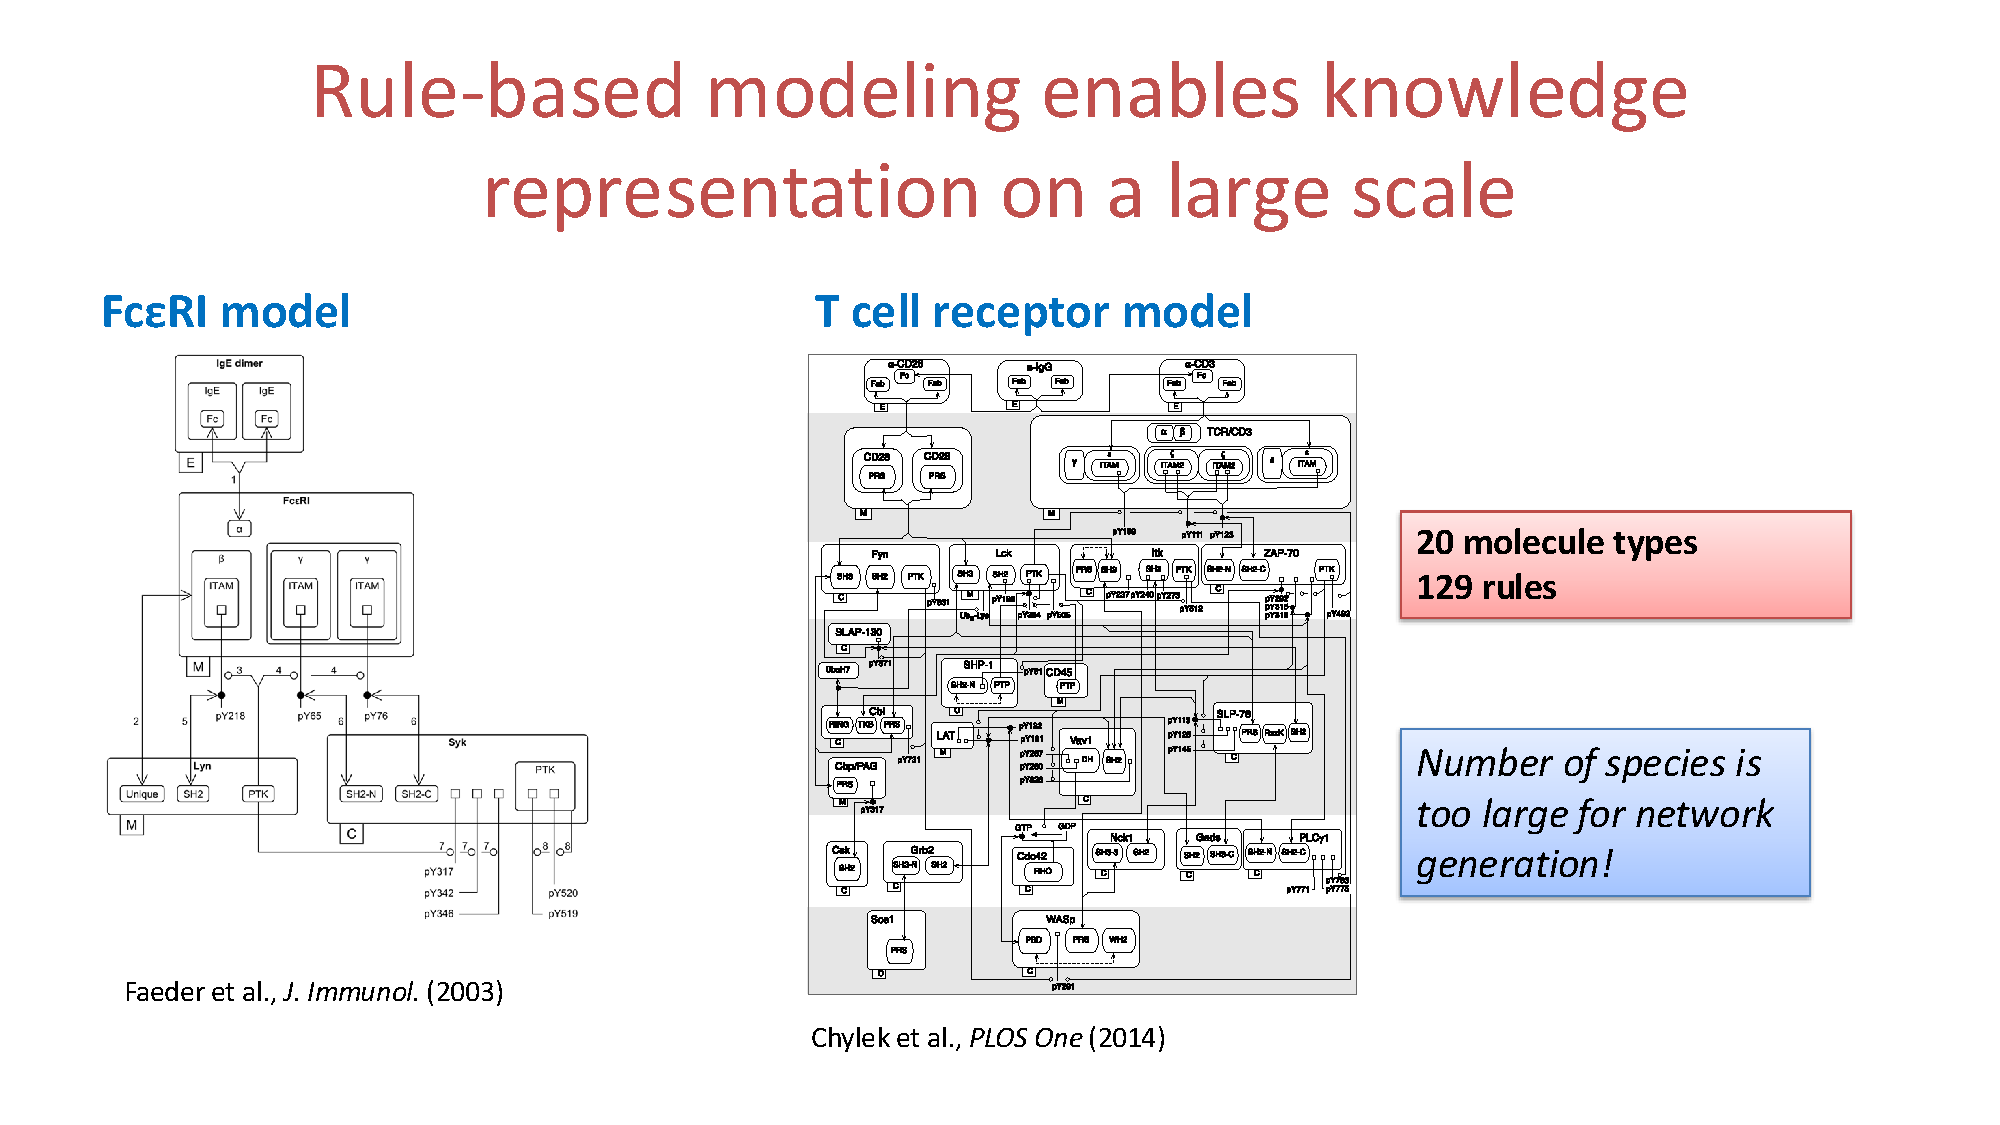
\includegraphics[width=\linewidth,trim=370 54 65 135,clip]{tcr_fceri_models.pdf}
    \end{column}
    \begin{column}{0.38\textwidth}
      \small
      A rule-based model of T cell receptor signaling: 20 molecule types and 129 rules.
      \vskip2mm
      The number of possible species is too large to enumerate, so the network
      cannot be generated at all.
      \vskip2mm
      Rule-based models also serve as precise, extensible, visualizable
      representations of what is known about a pathway.
    \end{column}
  \end{columns}
  \source{Chylek et al., \emph{PLOS One} (2014)}
\end{frame}

\begin{frame}{Two ways to simulate a rule-based model}
  \begin{columns}[c]
    \begin{column}{0.56\textwidth}
      \centering
      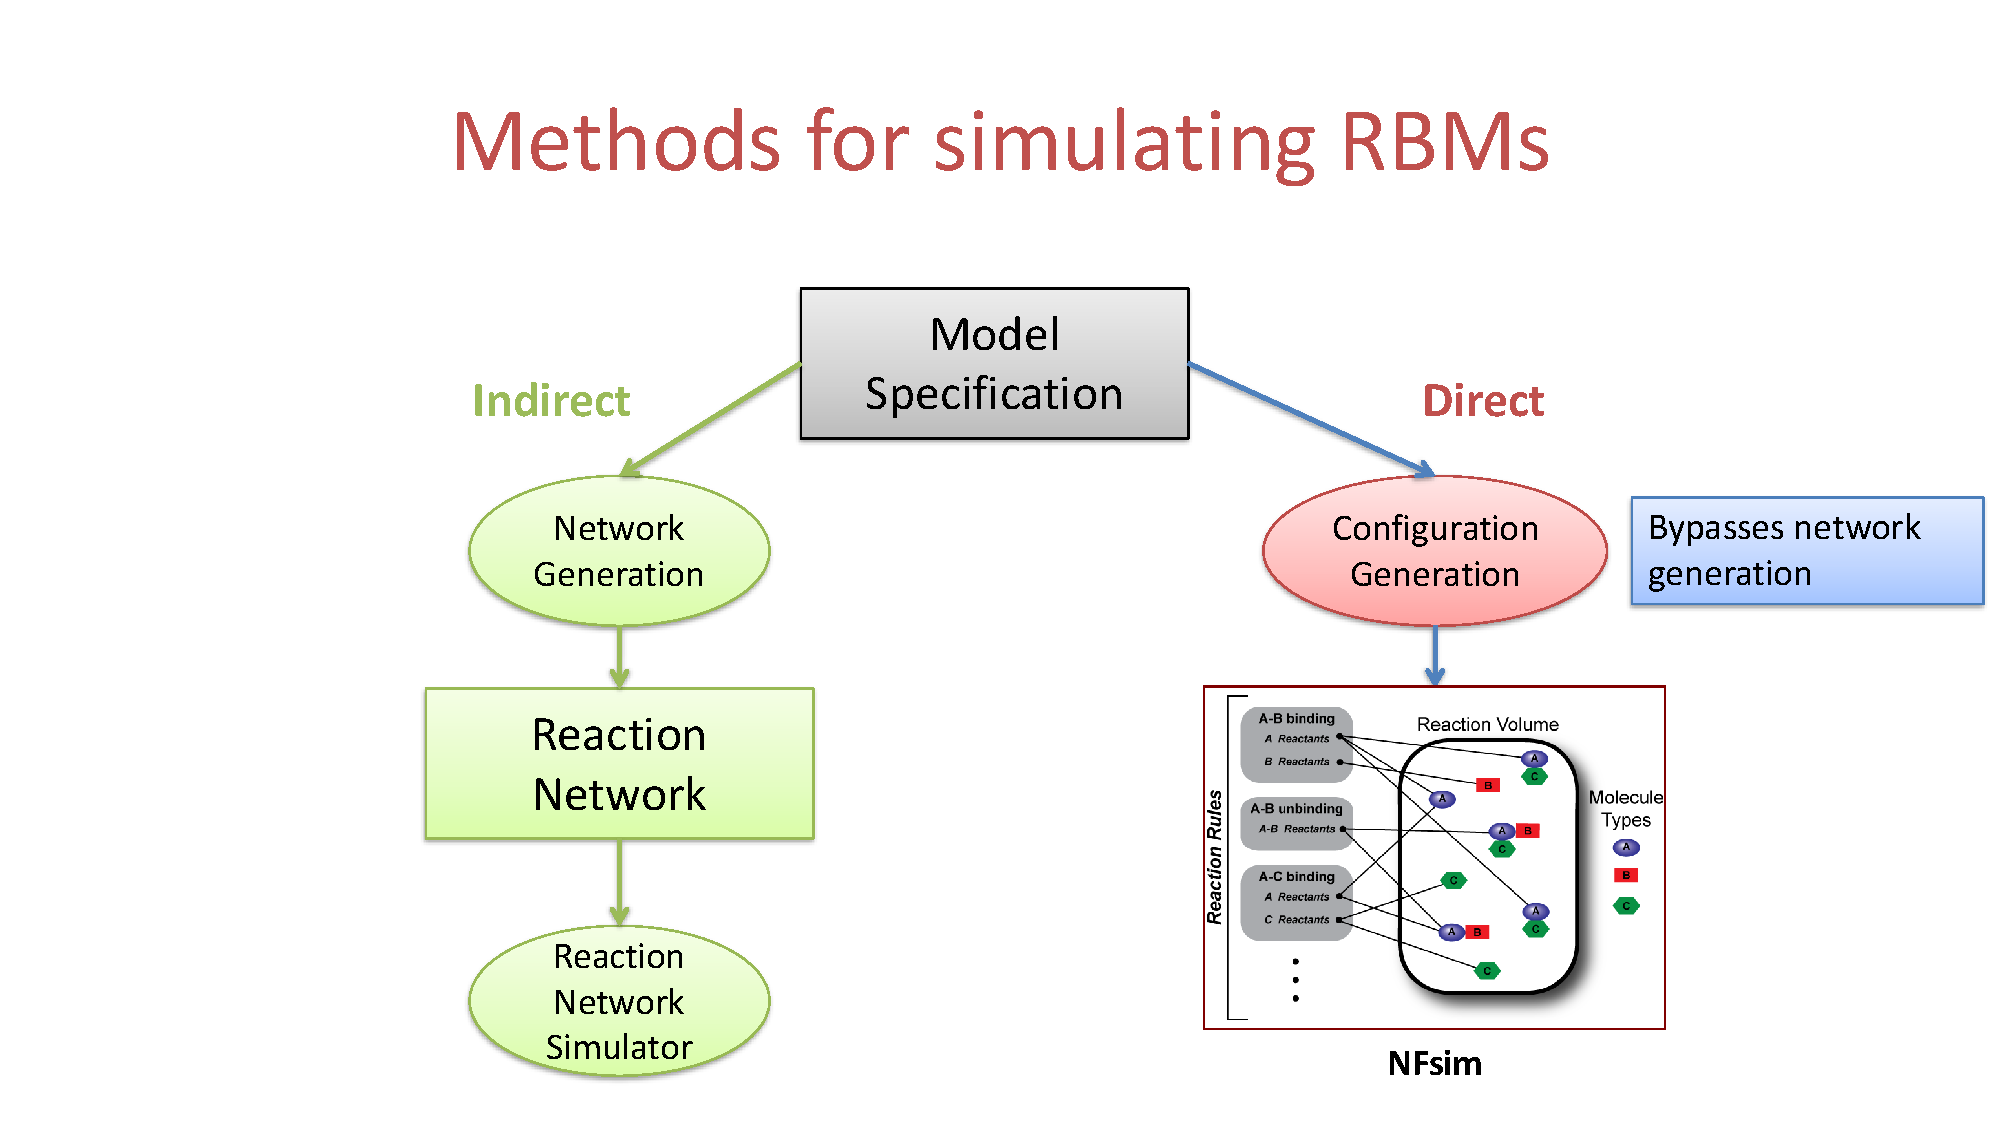
\includegraphics[width=\linewidth,trim=198 16 2 132,clip]{sim_methods.pdf}
    \end{column}
    \begin{column}{0.4\textwidth}
      \small
      \textbf{Indirect}: generate the network, then integrate ODEs or run SSA on it.
      Fast when the network is small. This is what we have done so far.
      \vskip2mm
      \textbf{Direct (network-free)}: track individual molecules and apply rules to
      them as the simulation runs. Only the complexes that actually form are ever
      represented.
      \vskip2mm
      \code{simulate(\{method=>"nf",...\})} runs NFsim.
    \end{column}
  \end{columns}
\end{frame}

\begin{frame}{Network-free simulation scales with the rules, not the network}
  \begin{columns}[c]
    \begin{column}{0.5\textwidth}
      \centering
      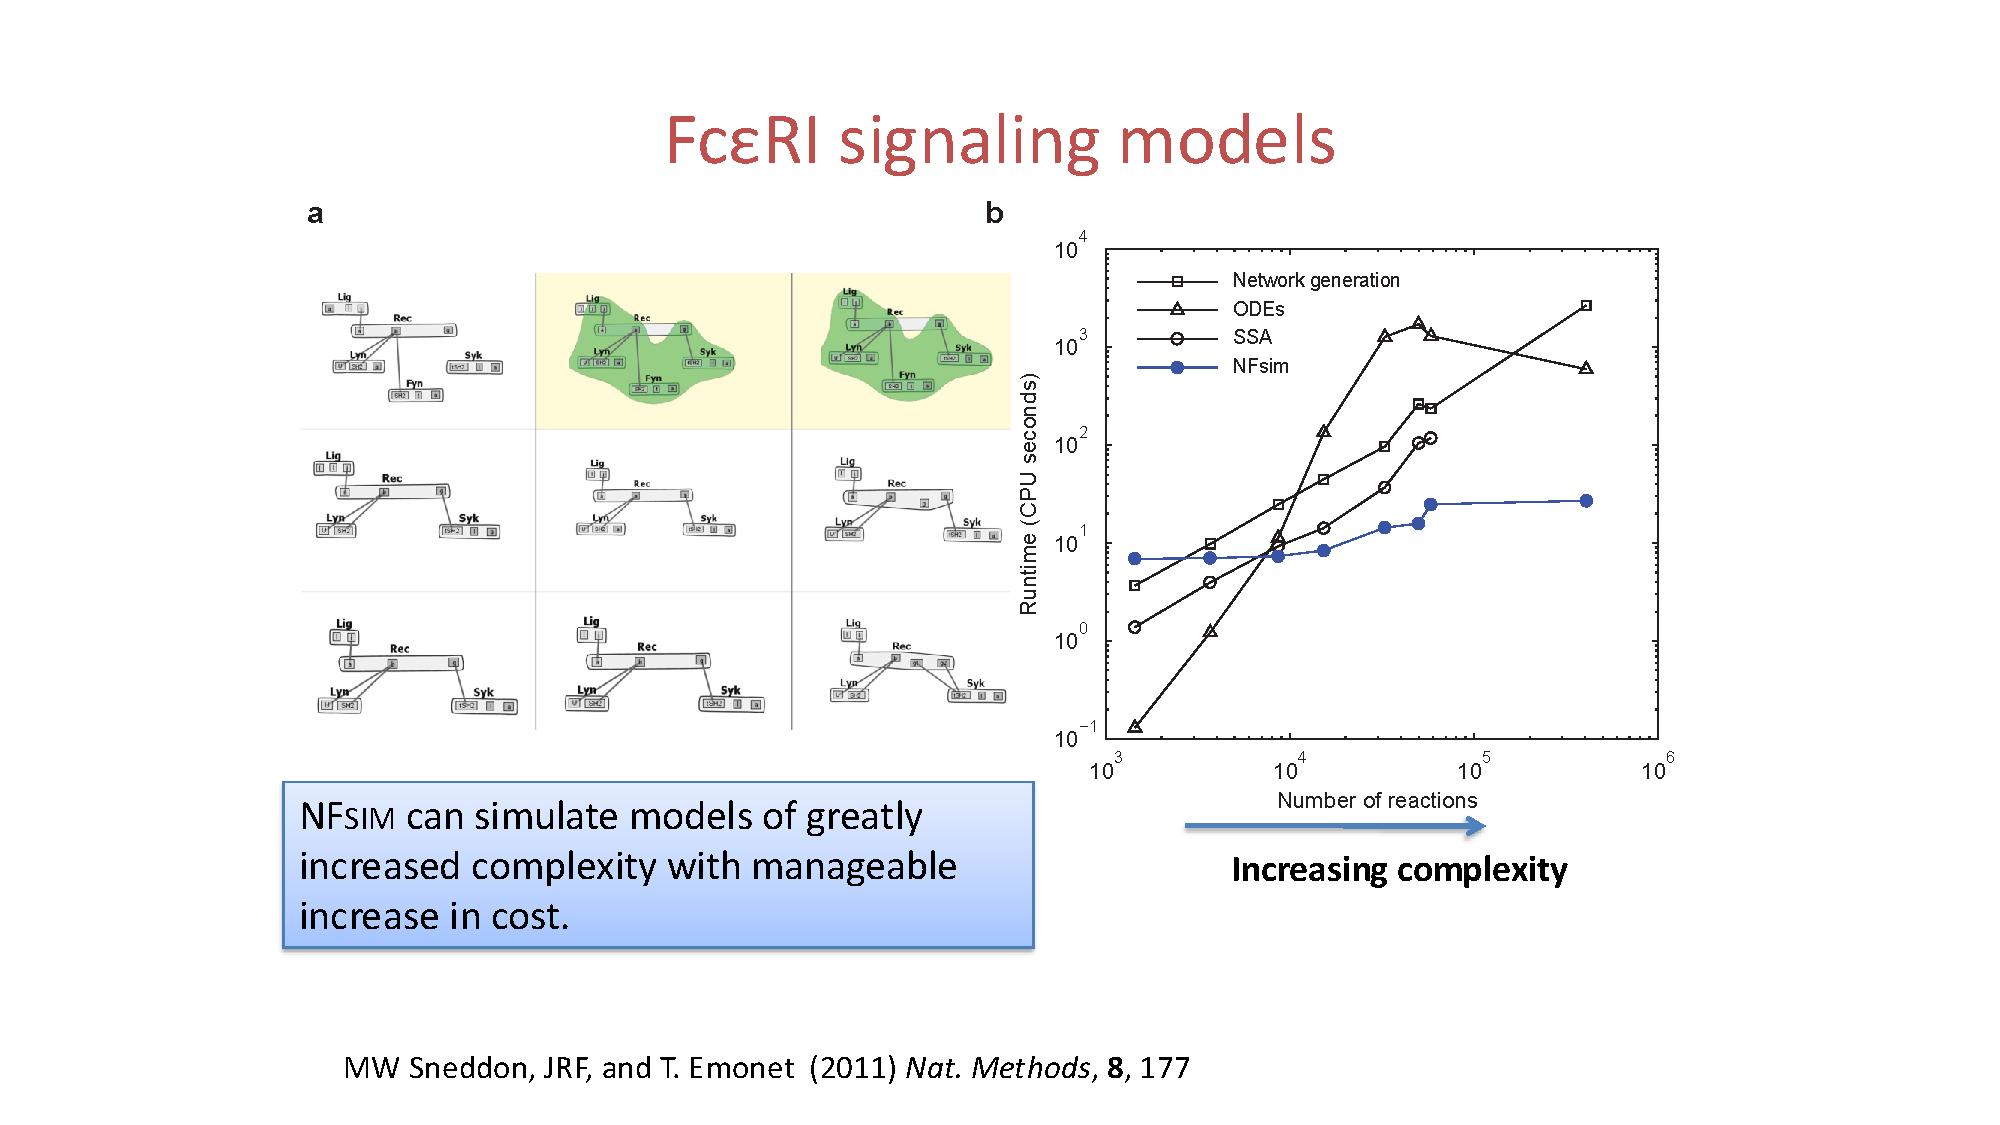
\includegraphics[height=0.68\textheight,trim=480 110 150 100,clip]{nfsim_scaling.pdf}
    \end{column}
    \begin{column}{0.46\textwidth}
      \small
      \begin{itemize}
        \setlength\itemsep{1.5mm}
        \item The cost of network generation and ODE integration grows with the
              number of reactions.
        \item NFsim's cost per event depends on the number of rules and molecules,
              so it handles models whose networks are huge or infinite.
        \item Trade-off: NFsim is stochastic and works with molecule counts, so results
              are noisy and concentrations must be converted to numbers.
      \end{itemize}
    \end{column}
  \end{columns}
  \source{Sneddon, Faeder, and Emonet, \emph{Nat.\ Methods} \textbf{8}, 177 (2011)}
\end{frame}

% ======================================================================
\begin{frame}{Try it yourself}
  Using \code{models/stat\_rbm*.bngl}:
  \begin{enumerate}
    \setlength\itemsep{1.5mm}
    \item In \code{stat\_rbm1\_rules.bngl}, change \code{R(l,s)} to \code{R(l)} in
          \code{LRbind}. Generate the network. Which new species appear, and why?
    \item Write an observable for receptors that carry both STAT and SOCS in
          \code{stat\_rbm3\_socs\_site.bngl}.
    \item In \code{stat\_rbm4\_receptor\_dimer.bngl}, vary \code{L0} from 0.01 to 100.
          Plot peak pSTAT against \code{L0}. Explain the shape.
    \item Remove the \code{r} context from \code{Sdimer} in
          \code{stat\_rbm5\_stat\_dimer.bngl} so receptor-bound pSTAT can dimerize.
          What happens when you generate the network? Try
          \code{generate\_network(\{max\_agg=>6\})}.
  \end{enumerate}
\end{frame}

\begin{frame}{Summary}
  \begin{itemize}
    \setlength\itemsep{2mm}
    \item Multi-site proteins create \textbf{combinatorial complexity}: a few
          interactions imply many species and reactions.
    \item BNGL represents molecules as objects with \textbf{components} (sites),
          \textbf{states}, and \textbf{bonds}; species are graphs.
    \item \textbf{Patterns} specify only what matters (don't write, don't care) and
          define observables that stay correct as the model grows.
    \item \textbf{Rules} transform patterns. One rule generates every reaction that
          fits its pattern; context restricts where it applies.
    \item BioNetGen \textbf{generates the network} from rules for ODE/SSA simulation;
          \textbf{NFsim} simulates models whose networks are too large to generate.
  \end{itemize}
\end{frame}

\end{document}
